\section{Methodology}
\label{sec:methods}

\subsection{Preprocessing}
\label{subsec:prepro}
The preprocessing of the images include: automatic selection of a region
of interest, image resampling to a resolution of $0.5 x 0.5 x 0.5$ mm, contours interpolation
using optical flow, bias correction using the N4ITK algorithm \cite{n4itk}, and
image normalization to an interval of [0,1].

The selection of the region of interested was proposed in \cite{anneke} and it 
consists of reducing the size of the three MRI series (axial, sagittal, and coronal)
by the intersection of its three corresponding rectangular prisms. The resampling
of the images is performed using linear interpolation with the ITK software \cite{itk}. 
The interpolation of the contours is performed in two dimensions fore each consecutives slices
of the contours. First, optical flow is obtained between the two slices using the  
Farneback method implementation in ITK. Then, the contours are modified following
the optical flow directions in a linear regression direction. Figure \ref{fig:of1} shows an
example of the resulting interpolated contour using the proposed method. 
\begin{figure}[h]
    \centering
    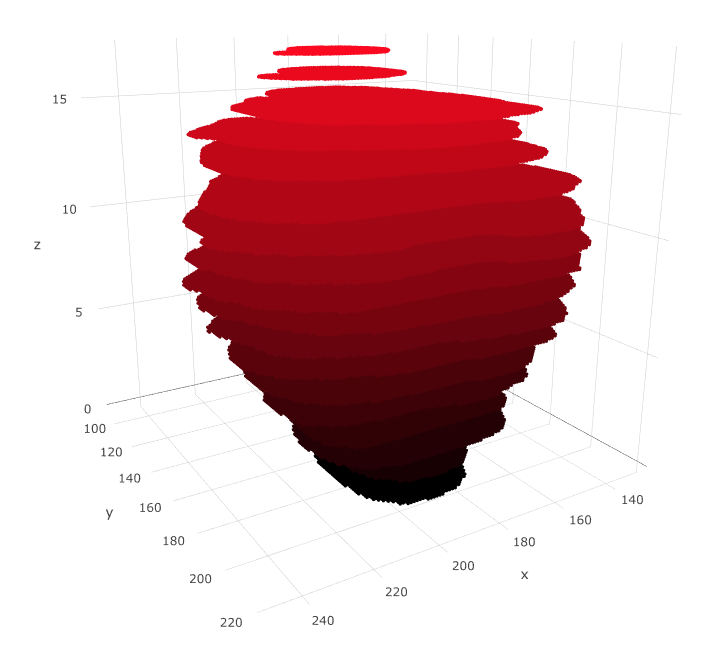
\includegraphics[totalheight=.15\textheight]{imgs/methodology/OF_1.png}
    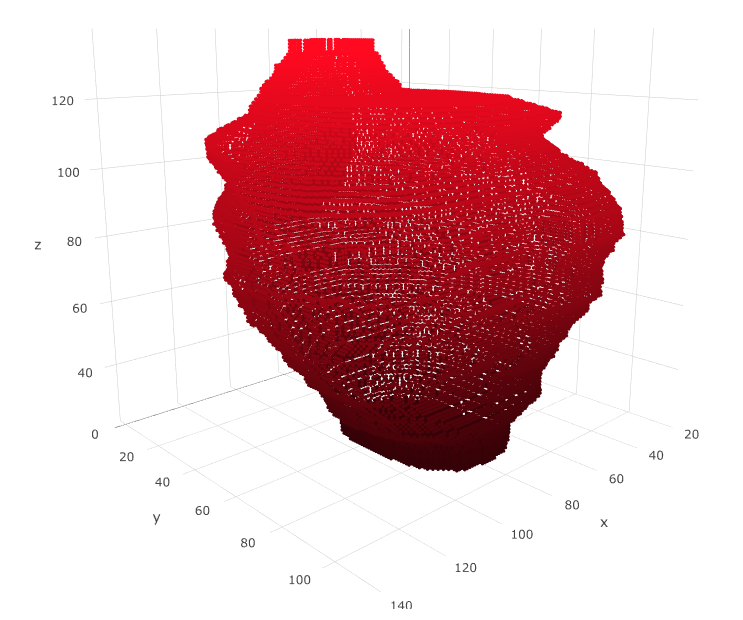
\includegraphics[totalheight=.15\textheight]{imgs/methodology/OF_2.png}
    \caption{Optical flow..}
    \label{fig:of1}
\end{figure}

\subsection{Proposed architecture}
The proposed 3D CNNs consists of a multistream encoding stage and a decoding stage. Each
of the mulstistream inputs receive an MRI image series of the ROI with a resolution of
$168^3$. The final ouput is a 

\begin{figure*}[h]
    \centering
    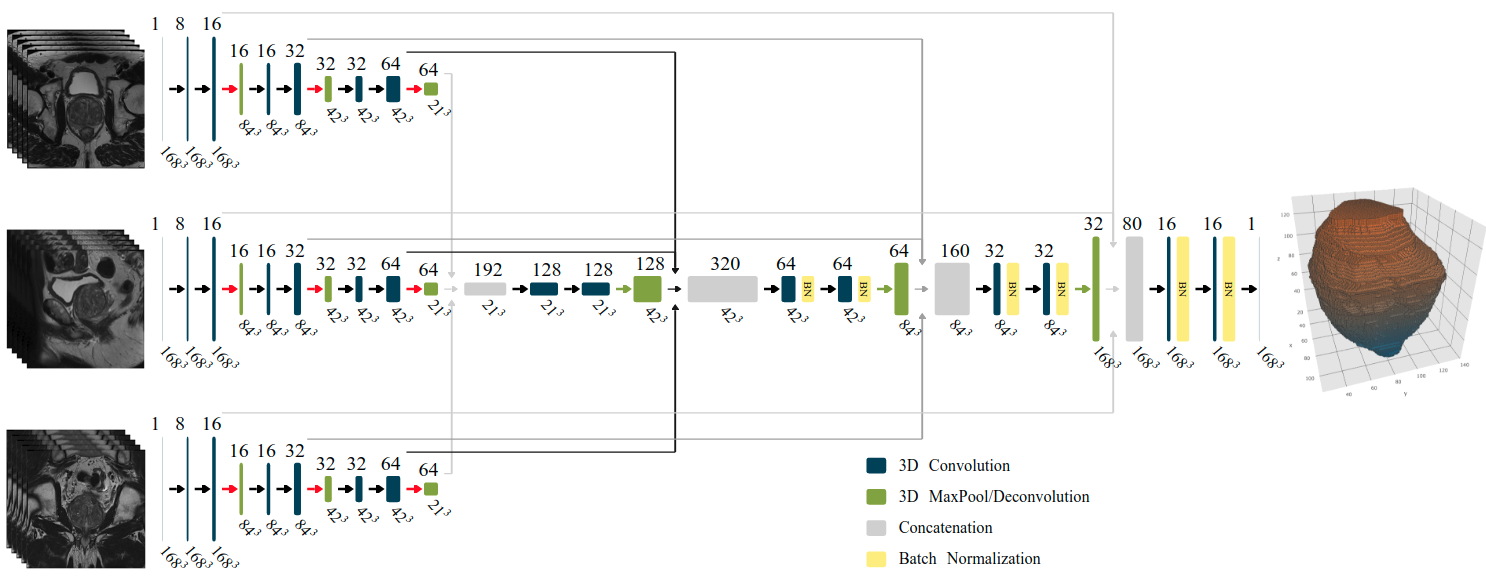
\includegraphics[totalheight=.3\textheight]{imgs/methodology/NN.png}
    \caption{Optical flow..}
    \label{fig:nn}
\end{figure*}
